\index{Schwender, Clemens}

\paragraph{Research Team}
Clemens Schwender (Professor), Thomas Jander (Student Assistant, Humbold University Berlin), Dr. Jens Ebert (Literature Historian), Elena Nedbaylo (PhD Candidate), Dr. Ortwin Buchbender (Military Historian)

 The Feldpost-Archiv is an archive for the war time generation's personal knowledge. Media are used to communicate experience, opinions, and knowledge. E-mails, letters, and the telephone are examples of individual media. The problem of investigating their content and usage is that they are usually not stored, but forgotten, deleted or thrown away - with one unique exception: Feldpost letters. With the Feldpost Collection, Feldpost letters will be catalogued and coded for scientific use. The data will be accessible over the Internet. The goal is to build a representative, web-based collection of war letters.

 Personal memories, experiences and written statements of the war generation are a valuable subject for research on memory and media, as well as for political psychology. Based on such collections, for instance, background questions about the age-graded effects of propaganda can be asked and hopefully answered in the near future. 

\begin{figure}[h]
  \begin{center}
    \begin{minipage}[b]{0.40\linewidth}
   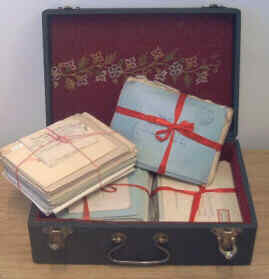
\includegraphics[width=\linewidth]{profClemensSchwender-fig2.jpg}
    \end{minipage}\hfill
    \begin{minipage}[b]{0.55\linewidth}
      \caption{Collection of letters in the Feldpost-Archiv in Berlin, initiated by Clemens Schwender.\label{fig2:profClemensSchwender}}
    \end{minipage}
  \end{center}
\end{figure}

\textbf{Research Highlights 2006}

 This year our work concentrated on a survey of so called ``gray literature''. These are publications and editions of war letters and memoirs by war participants or their relatives. Usually these are not critical editions and lack information on provenance. But nevertheless they are important for war letter research and provide a useful source of information if handled with care.

%\begin{figure}[ht]
%  \begin{center}
%    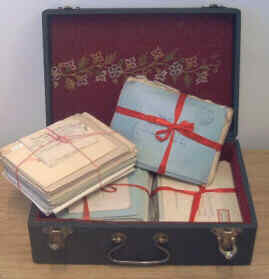
\includegraphics[width=7.5cm]{profClemensSchwender-fig2.jpg}
%    \caption{Collection of letters in the Feldpost-Archiv in Berlin, initiated by Clemens Schwender.}\label{fig2:profClemensSchwender}
%   \end{center}
%\end{figure}

\paragraph{Collaborations}
\begin{itemize}
\item Museum of Communication Berlin \\ Prof. Dr. Joachim Kallinich
\item State Library Stuttgart \\ Prof. Dr. Gerhard Hirschfeld
\item Prussian Cultural Heritage in Berlin, State Library \\ Dr. Jutta Weber 
\item University of Witten/Herdecke \\ Prof. Dr. Harald Welzer
\item State University Surgut, Russia \\ Dr. Vasiliy Glushak
\end{itemize}

\begin{bibunit}[apalike]
\nocite{*}
\putbib[profClemensSchwender3]
\end{bibunit}